\begin{titlepage}
	\begin{center}
		\chapter{Les rôles de \textbf{IA} dans la médecine}
		\minitoc

		\vspace{5cm}
		\pgfspectra[element=He,absorption]
	\end{center}
	\vfill % Remplir le reste de la page avec du blanc
\end{titlepage}
\pagestyle{monstyle}\setcounter{page}{5}

\section{Introduction}
  \begin{itemize}
        \item L'IA, par les algorithmes, aide donc principalement à l'élaboration de
              diagnostics.
        \item En effet, la machine prescrit le même diagnostic que les
              médecins dans 99\% des cas, et dans 30\% des cas, elle propose un
              traitement plus adapté que celui des spécialistes. Elle réussit à
              détecter les cancers du sein dans 89\% des cas, alors que les
              spécialistes les détectent dans 73\% des cas.
        \item Ainsi, la robotique étend sa toile dans de nombreux secteurs de
            la médecine.
  \end{itemize}
\section{Les rôles de \textbf{IA} dans la médecine}

\begin{itemize}
        \item les prothèses intelligentes
            \medskip
            \compo[0.7]{
                Des systèmes basés sur l'intelligence artificielle et la
                reconnaissance ou le diagnostic de formes, qui donneront
                aux paraplégiques la capacité de se tenir debout ou de
                monter des escaliers. Les lunettes permettent aux
                personnes aveugles d'identifier des objets ou des
                personnes ou même de lire un texte.\\

                De nombreuses applications nécessitent des algorithmes complexes
                et d'énormes quantités de calculs. De plus, de très
                grandes bases de données, correctement annotées, sont
                indispensables pour permettre un apprentissage précis et
                ainsi la création de prothèses aussi efficaces que des
                membres humains.            
                \\[1cm]
            }{
                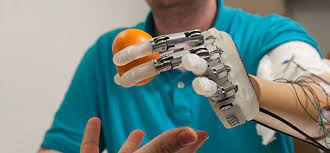
\includegraphics[height=\textwidth,width=\textwidth]{photo/prothese.jpg}
            }
        \item 
            les traitements personnalisés grâce au recoupement
            de données (big data)… 
            \medskip
            \compo[0.7]{
                Objectif de la médecine personnalisée :
                faire le bon diagnostic pour adresser le bon traitement, au bon
                moment, au bon patient. \\

                Cette approche innovante est
                portée par les dernières avancées scientifiques et
                technologiques qui permettent de collecter et de décrypter
                les données génomiques1 des patients et de leurs maladies.\\

                En s’appuyant sur l'analyse du génome, les soignants sont
                dorénavant en mesure de mieux prédire la réponse du
                patient au traitement qui lui sera proposé, en écartant
                par la même occasion un certain nombre d’effets
                secondaires qu'ils n’auraient pas pu anticiper avec un
                traitement dit conventionnel. \\[1cm]
            }{
              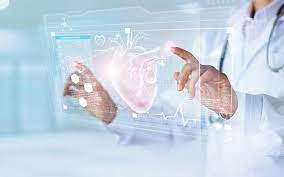
\includegraphics[height=\textwidth,width=\textwidth]{photo/cardio.jpg}
            }


        \item Reconnaissance d'images pour le diagnostic du cancer;\\[0.1cm]

                Des algorithmes d'apprentissage en profondeur liés à la
                reconnaissance de formes dans les images ont été
                développés pour simuler la reconnaissance visuelle par
                ordinateur.\\

                Ces algorithmes, connus sous le nom de réseaux
                de neurones convolutifs, miment la vision par le fait
                qu'ils s'efforcent de reproduire la vision en
                reconstruisant une image tout comme le font les neurones
                de la rétine pour propager l'information d'une image dans
                le cerveau.\\

                Les premières couches de neurones extraient
                les caractéristiques structurelles de l'image, puis les
                caractéristiques de ces structures sont propagées dans les
                couches intermédiaires de neurones tout en conservant
                leurs hiérarchies structurelles.\\

                Enfin, les informations sont agrégées dans la dernière couche de neurones pour
                prédire une décision de reconnaissance de formes dans
                l'image. \\[0.25cm]

        \item amélioration de la prestation des soins de santé: \\[0.1cm]

            L'IA transforme la façon dont nous prenons soin de
            nous. Voici trois façons dont l'IA transforme déjà la
            prestation des soins médicaux.

            \medskip
            \begin{itemize}
                \item[-] Recommandations de traitement.
                \item[-] Participation du patient et observance thérapeutique.
                \item[-] Simplifie les tâches administratives.
                    \\[0.25cm]
            \end{itemize}

        \item le suivi des patients à distance,
            \\[0.25cm]

        \item Diagnostique:\\[0.1cm]

                la comparaison entre différentes modalités d'imagerie une
                échographie antérieure et un examen d'imagerie par résonance
                magnétique \\[0.25cm]

        \item Médecine prédictive\\[0.1cm]

                Prédire une lésion rénale 48 heures avant! C'est possible grâce à 
                ``Deep Learning'', grâce à une société d'intelligence artificielle qui
                a développé un algorithme capable de détecter des marqueurs
                biologiques annonciateurs des lésions rénales. ce qui permettrait de
                réduire de 11 \% les décès dus à ce genre d'événement.\\

                L'IA serait aussi capable de prédire la maladie d'Alzheimer en analysant des
                images cérébrales ou un échantillon sanguin, et même des accidents
                cardiaques en fonction d'un électrocardiogramme $(ECG)$. \\[0.25cm]

        \item Nouveaux médicaments\\[0.1cm]

            En passant au crible des milliards de molécules, l'intelligence
            artificielle est capable de prédire celles qui vont correspondre à un
            récepteur de cellule ou d'un virus.
            En juillet 2019, une équipe
            australienne a ainsi conçu le premier vaccin doté d'un adjuvant trouvé
            par un algorithme.\\

            L'IA permet d'élargir le champ des
            candidats-médicaments à des molécules que les chercheurs ne
            soupçonnaient pas, et de mieux anticiper les effets secondaires des
            futurs médicaments. \mybox


\end{itemize}
